\documentclass[11pt,a4paper]{article}
\usepackage[margin=2.5cm]{geometry}
\usepackage{booktabs}
\usepackage{listings}
\usepackage{xcolor}
\usepackage{graphicx}
\usepackage{float}

\lstset{
  basicstyle=\ttfamily\small,
  frame=single,
  backgroundcolor=\color{gray!8},
  breaklines=true
}

\title{Labwork 9: Histogram Equalization}
\author{Yanis Denizot -- 2640051}
\date{\today}

\begin{document}
\maketitle

\section{Implementation}
Like in labwork 7, I used a low contrast version of the image (\texttt{img * 0.4 + 80}, values
between 80 and 182) so the effect is visible. The image is $1200 \times 800$ and I used Google
Colab (Tesla T4). The image is first converted to gray with a 2D map kernel.

\textbf{9a: Histogram.} If all the threads do \texttt{histo[gray] += 1} at the same time, they
write the same bins and some counts are lost (race condition). We have not seen atomic
operations yet, so I used local histograms, like in the course:
\begin{itemize}
  \item Gather: one thread per row of the image. Each thread reads its 1200 pixels and counts
        them in its own histogram (one row of a $800 \times 256$ array), so there is no conflict.
  \item Reduction: one thread per bin (256 threads). Thread \texttt{b} adds bin \texttt{b} of
        the 800 local histograms.
\end{itemize}
\begin{lstlisting}[language=Python]
@cuda.jit
def local_hist(gray, lhist):
    row = cuda.threadIdx.x + cuda.blockIdx.x * cuda.blockDim.x
    if row < gray.shape[0]:
        for x in range(gray.shape[1]):
            lhist[row, gray[row, x]] += 1

@cuda.jit
def sum_hist(lhist, hist):
    b = cuda.threadIdx.x + cuda.blockIdx.x * cuda.blockDim.x
    if b < 256:
        s = 0
        for r in range(lhist.shape[0]):
            s += lhist[r, b]
        hist[b] = s
\end{lstlisting}

\textbf{9b: Equalization.} The histogram (256 values) is copied to the CPU. Then, in sequential
like asked in the course, I compute the probability $p_j = histo_j / n$, the cumulative
distribution $c_i = \sum_{j=0}^{i} p_j$, and a lookup table $lut[i] = c_i \times 255$ (rounded).
This is only 256 steps. The table is sent to the GPU, and a 2D map kernel replaces each pixel by
\texttt{lut[pixel]}, which is also a gather (reading the table at the index given by the pixel).
\begin{lstlisting}[language=Python]
def make_lut(hist):
    n = hist.sum()
    lut = np.zeros(256, np.uint8)
    c = 0.0
    for i in range(256):
        c = c + hist[i] / n
        lut[i] = int(c * 255 + 0.5)
    return lut
\end{lstlisting}

\section{Results}
The GPU histogram is the same as the CPU histogram, and the equalized image is the same as the
CPU result (maximum difference = 0).

\begin{figure}[H]
\centering
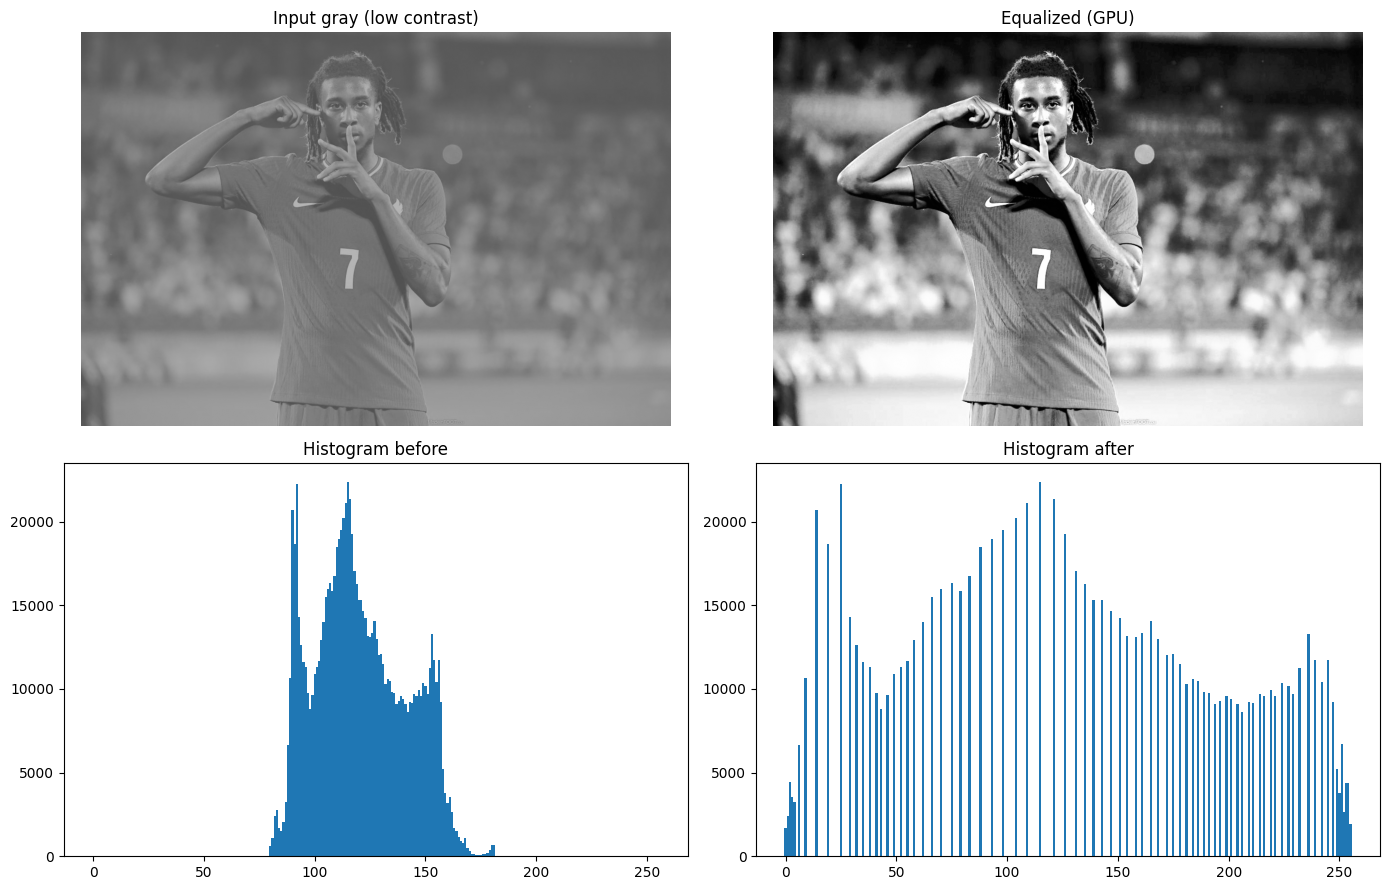
\includegraphics[width=0.9\textwidth]{results.png}
\end{figure}

Before, all the gray values are between 80 and 182. After equalization they are spread from 0
to 255 and the image has much more contrast. The histogram after has gaps: the input has only
about 100 different gray values, and they are mapped to 256 possible values, so some values are
never used. The height of the bars stays the same, only their position changes.

\begin{table}[H]
\centering
\begin{tabular}{lr}
\toprule
& Time \\
\midrule
CPU (Python loops) & 2.44 s \\
GPU (full pipeline, average of 20 runs) & 1.97 ms \\
\midrule
Speedup & 1235 \\
\bottomrule
\end{tabular}
\end{table}

The speedup is lower than for the map kernels of the previous labworks. The local histogram
kernel uses only 800 threads (one per row, 13 blocks of 64), which is not enough to use the whole
GPU (Numba also gives a warning about it), and each thread reads 1200 pixels one by one. Also,
the threads of a warp read pixels in different rows, so the memory accesses are not coalesced.
The pipeline also copies the histogram to the CPU and the table back to the GPU.

\end{document}
